\documentclass[conference, compsocconf, letterpaper]{IEEEtran}

\usepackage[utf8]{inputenc} % set input encoding (not needed with XeLaTeX)

%%% PAGE DIMENSIONS
%\usepackage{geometry} % to change the page dimensions
%\geometry{a4paper} % or letterpaper (US) or a5paper or....
% \geometry{margins=2in} % for example, change the margins to 2 inches all round
% \geometry{landscape} % set up the page for landscape
%   read geometry.pdf for detailed page layout information

\usepackage{graphicx} % support the \includegraphics command and options

% \usepackage[parfill]{parskip} % Activate to begin paragraphs with an empty line rather than an indent

%%% PACKAGES
\usepackage{booktabs} % for much better looking tables
\usepackage{array} % for better arrays (eg matrices) in maths
\usepackage{paralist} % very flexible & customisable lists (eg. enumerate/itemize, etc.)
\usepackage{verbatim} % adds environment for commenting out blocks of text & for better verbatim
\usepackage{subfig} % make it possible to include more than one captioned figure/table in a single float
% These packages are all incorporated in the memoir class to one degree or another...
\usepackage{algorithm}
\usepackage{algpseudocode}
\usepackage{amsthm}

%%% HEADERS & FOOTERS
\usepackage{fancyhdr} % This should be set AFTER setting up the page geometry
\pagestyle{fancy} % options: empty , plain , fancy
\renewcommand{\headrulewidth}{0pt} % customise the layout...
\lhead{}\chead{}\rhead{}
\lfoot{}\cfoot{\thepage}\rfoot{}

%%% SECTION TITLE APPEARANCE
%\usepackage{sectsty}
%\allsectionsfont{\sffamily\mdseries\upshape} % (See the fntguide.pdf for font help)
% (This matches ConTeXt defaults)

%%% ToC (table of contents) APPEARANCE
%\usepackage[nottoc,notlof,notlot]{tocbibind} % Put the bibliography in the ToC
%\usepackage[titles,subfigure]{tocloft} % Alter the style of the Table of Contents
%\renewcommand{\cftsecfont}{\rmfamily\mdseries\upshape}
%\renewcommand{\cftsecpagefont}{\rmfamily\mdseries\upshape} % No bold!

%%% END Article customizations

%%% The "real" document content comes below...

\title{Map Reduce on a Chord Distributed Hash Table}
\author{
Andrew Rosen \qquad Brendan Benshoof \qquad Matt Erwin \qquad Robert Harrison \qquad Anu Bourgeois  \\Department of Computer Science, Georgia State University\\ 34 Peachtree St NW \\ Atlanta, Georgia 30303\\  rosen@cs.gsu.edu }
%\date{} % Activate to display a given date or no date (if empty),
         % otherwise the current date is printed 

\begin{document}
\maketitle

\begin{abstract}

Large problems in Computer Science are often able to be split into many smaller, functionally identical tasks, the results of which can be reduced into the desired solution.  MapReduce is a framework for 
performing distributed computations of these types of problems, but most of these frameworks are strongly dependent on a heirarchical structure.  Chord is a distributed hash table that provides $\log_{2}n$ connectivity among processors.  Our experiments show that a Chord ring has number of desirable advantages for implementing MapReduce, such as a lack of a single point of failure, fault-tolerance, an even distribution of work, scalability, and minimal overhead.
%Distributed Hash networks, such as Chord, are an established technique for storing data in a distributed fashion. In Chord, nodes are evenly distributed and are responsible for files based on their position in the overlay network.  From Chord, we introduce the concept of the Hashnet, where computers use distributed hash table as a means of distributing both data and work.  Because Chord provides the backbone of this network, a Hashnet is robust, scalable, resilient to churn, fault tolerant, and automatically  and evenly distributes work throughout the network.

%We can exploit this property to automatically distribute large and complicated tasks, such as MapReduce, evenly among nodes in the same manner. Our experiments show that our framework distributes work among nodes in manner that is highly scalable, resilient to churn, and fault tolerant.

%HARRISON:  Map reduce is a family of algorithms for distributed computations. The basic idea with these algorithms is to factor a large task into independent tasks that can be mapped to a set of processors and the have the results reduced back to the desired solution. Chord networks are a ring of processors with a log(n) connectivity.  In this paper we show that the chord network has advantages for implementing map/reduce because of its low latency (low overhead?) connectivity. (you probably can state this better than me).
\end{abstract}

TODO GO THROUGH AND UNIFY TERMINOLOGY:  MAPREDUCE TASK/JOB

RELATED WORK MIGHT BE BETTER PLACED NEAR CONCLUSION

CAPITALIZE ALL MAPS AND REDUCES

ADD WHAT CHRONUS STANDS FOR

CHECK FORMATTING MATCHES WHAT THEY WANT FOR SUBMISSION

\section{Introduction}

Ever since Google published a paper on the subject \cite{mapreduce}, MapReduce has rapidly become an integral part in the world of data processing.  Using MapReduce, a user can take a large problem, split it into small, equivalent parts and send those parts off to be worked on by other processors.  These results of these computations are then sent back to the user and combined until one large answer results.  Numerous programming tasks - word counts, reverse indexing, sorting, Monte-Carlo approximations - can be efficiently distributed using MapReduce \cite{mapreduce}.

The most popular platform for MapReduce is Hadoop \cite{Hadoop}. Hadoop is an open-source Java implementation deveolped by Apache and Yahoo! \cite{pavlo2009comparison}.  Haddop has two components, the Hadoop Distributed File System (HDFS) and the Hapdoop MapReduce Framework \cite{mrsurvey}.  Under HFDS, nodes are arranged in a heirarchical tree, with a master node, called the NameNode, at the top.  The NameNode is responsible for keeping track of whcih DataNodes posess which files, as well as coordinating the work done under a MapReduce job \textsuperscript{\textbf{double check the latter}}. 
 
However, what if we desire a less heirarchical structure among our nodes?  A single node in charge is a single point of failure.  We need a system that can scale, is fault tolerant, has a minimal amount of latency, and distributes files evenly. 

Chord \cite{Chord} is a distributed hash table (DHT) that possesses these qualities.  Chord guarantees a worst-case $\log n$ lookup time for a particular node or file in the network. It is highly fault-tolerant to node failures and churn.  It scales extremely well and there is little maintenance required by the network as a whole to handle individual nodes.  Files in the network are distributed evenly among its members.
 
However, rather that viewing Chord solely as a means for sharing files, we see it as a means for distributing work.  We have developed a system, called CHRONUS, that builds off the concepts that make Chord a powerful means of evenly distributing files and applies it toward distributing work among member nodes\footnote{repetitive}.  We built a framework on CHRONUS for performing Map and Reduce tasks on Chord ring.  CHRONUS leverages the underlying protocol to distribute map and reduce tasks to nodes evenly, provide greater data redundancy, and guarantee a greater amount of fault tolerance.  The network has no single point of failure.

At the same time we avoid the architectural and file system constraints of systems like Hadoop.  Nodes in CHRONUS can be setup in a cluster for high performance or they can be deployed the Internet, for volunteer computing tasks.  Our experiments demonstrate that our framework is highly scalable, solving problems significantly faster when distributed.  The larger the problem is, the greater the speedup gained by incorperating more nodes into the problem.  Our framework also provides a high level of robustness during execution;  we can lose any node to churn and still process jobs successfully\footnote{Brendan, check}.


Section X covers the specifics of the Chord Protocol and the design choices we made for implementation. We describe MapReduce and Hadoop in more detail in Section QA4162.  Related Work is discussed in Section 42. Details of CHRONUS's implementation and code is described in Section Q, while our experiments and their results are covered in Section Z.  Lastly, Section L discusses fruitful avenues of future research.

%\subsubsection{Current models of distributing work}
%Talk about hadoop mention how we basically have a way to distribute reduce.
%Hadoop is popular here's a citation.  Popular enough to justify using it as a means of comparison

%\subsubsection{HFDS}
%Hadoop is strongly tied to HFDS architecture.  We are tied to having a computer.

%\subsubsection{Our proposed model Hashnet:  A system of computers connected together using a distributed hash table as a means for efficiently distributing both data and work.}

%A hashnet is not a new paradigm for distributing work; it is an extension of the established and highly tested means of distributing files and applying the scheme to do the same for work.



\section{CHORD}
The Chord protocol \cite{Chord} takes in some key and returns the identity (ID) of the node responsible for that key.  These keys are generated by hashing a value of the node, such as the IP address and port, or by hashing the filename of a file.  The hashing process creates a $m$-bit hash identifier.

The nodes are then arranged in a ring from the lowest hash-value to highest.  Chord then takes the hashed files and places each in the node that has the same hashed identifier as it.  If no such node exists, the node with the first identifier that follows this value.  This node responsible for the key $\kappa$ is called the $successor$ of $\kappa$, or $successor(\kappa)$.  Since the overlay is a circle, this assignment is computed in module $2^m$ space.  For example, if there were some portion of the network with nodes 20, 25, and 27, node 25 could be responsible for the files with the keys (21,22,23,24,25). If node 25 were to decide to leave the network, it would inform node 27, who would then be responsible for all the keys node 25 was covering. An example Chord network is drawn in in Figure INSERT FIG HERE.

With this scheme, we can reliably find the node responsible for some key by asking the next node in the circle for the information, who would then pass the request through the circle until the successor was found.  We can then proceed to directly connect with the successor to retrieve the file.  This naive approach is largely inefficient, and is a simplification of the lookup process, but it is the basis of how Chord theoretically works.

To speed up the lookup time, each node builds and maintains a \emph{finger table}.  The \emph{finger table} contains the locations of up to $m$ other nodes in the ring.  The $i$th entry of node $n$'s \emph{finger table} corresponds to the node that is the $successor(n+2^{i-1})$ $mod$ $2^m$. Because hash values won't be perfectly distributed, it is perfectly acceptable to have duplicate entries in the \emph{finger table}. 


\begin{figure}
    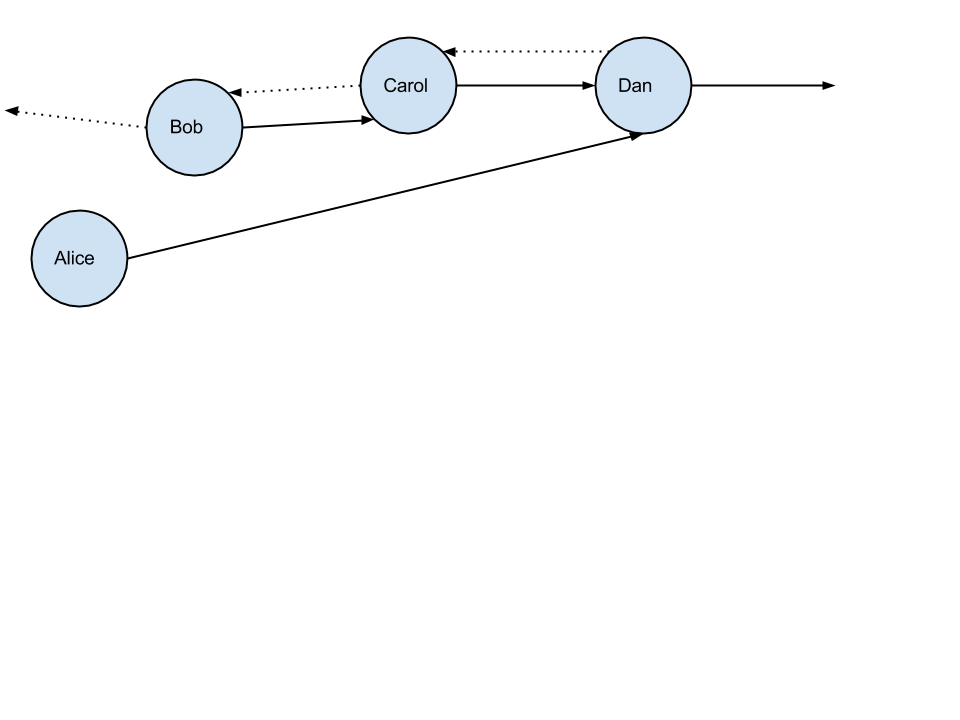
\includegraphics[width=\linewidth]{abcd1}
    \caption{Alice has incorrectly determined that Carol is her appropriate successor.  When Alice stabilizes, Carol will let her know about Bob.}
    \label{abcd1}
\end{figure}


\begin{figure}
    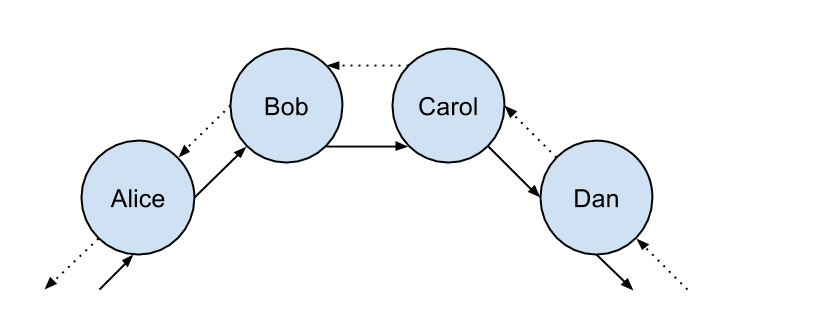
\includegraphics[width=\linewidth]{abcd2}
    \caption{After completing stabilize, Alice makes Bob her successor and notifies him. Bob then made Alice as his predecessor.}
    \label{abcd2}
\end{figure}



When a node $n$ is told to find some key, $n$ looks to see if the key is between $n$ and $successor(n)$ and return $successor(n)$'s information to the requester. If not, it looks for the entry in the finger table for the closest preceding node $n'$ it knows and asks $n'$ to find the successor.  This allows each step in the to skip up to half the nodes in the network, giving a $\log_2(n)$ lookup time.  Because nodes can constantly join and leave the network, each entry in the table is periodically checked and updated. 

To join the network, node $n$ first asks $n'$ to find $successor(n)$ for it.  Node $n$ uses the information to set his successor, but the other nodes in the ring will not acknowledge $n$'s presence yet.  Node $n$ relies on the stabilize routine to fully integrate into the ring.

The stabilize routine helps the network integrate new nodes and route around nodes who have left the networls. Each node periodically checks to see who their successor's predecessor is.  In the case of a static network, this would be the checking node.  However, if the checking node gets back a different node, it looks at that returned node's hash value and changes their successor if needed.  Regardless of whether the checking node changes its successor, that node then notifies the ( possibly) new successor,  essentially telling the successor "based on the information I have, I'm your predecessor.  Check to see if you need to update your predecessor information," to which the successor obliges.  A more concrete example:


Suppose Alice, Bob, Carol, and Dan are members of the ring and everyone happens to be ordered alphabetically (Figure \ref{abcd1}). Alice is quite sure that Carol is her successor.  Alice asks Carol who her predecessor is and Carol says Bob is.  Since Bob is closer than Carol, Alice changes her successor to Bob and notifies him.  

When Bob sees that notification, he can see Alice is closer than whoever his previous predecessor is and sets Alice to be his predecessor.  During the next stabilization cycle, Alice will see that she is still Bob's predecessor and notify him that she's still there (Figure \ref{abcd2}).

One of the major design choices for Chord implementation is not figuring which node is responsible for a given key, but figuring out who decides which node is responsible for a given key.  In our implementation, a node $n$ is responsible for the keys ($predecessor(n)$, $n$].  In other words, when $n$ gets a message, it considers itself the intended destination for the message if the message's destination hash is between $predecessor(n)$ and $n$.  A node that does not have a predecessor assigns itself as its own predecessor and considers itself responsible for all messages it receives. 

When a node $n$ changes his successor, $n$ asks if the successor is holding any data $n$ should be responsible for.  The successor looks at all the data $n$ is better suited to hold onto, packages it up, and sends it along to $n$.  The successor does not have to delete this data. If fact, keeping this data as a backup is beneficial to the network as a whole, as $n$ could decide to leave the network at any point. 

Due to the potentially volatile nature of a peer-to-peer network, Chord has to be able to handle (or at the very least, tolerate) an arbitrary amount of churn.  We already detailed how Chord gradually guides nodes into their correct locations after they join the network.  The same is true for when a node leaves the network; the stabilize procedure will guide nodes to their correct successors and predecessors.  However, we can exert more control over how to handle nodes leaving the network

A node can leave the ring in one of two ways.  A node can either suddenly drop out of existence, or a node can tell the network he is about to leave, letting his successor and predecessor immediately perform the needed changes.

When a node politely quits, he informs both his successor and predecessor and gives them all the information they need to fill the gap that would be left over. He also sends all of the data he is responsible for to his successor, who would become responsible for that data when that node left.  Fingers that pointed to that node would be corrected during the finger maintenence period.  This allows for the network to adjust to the change with a minimum of fuss.

Unfortunately, it is impossible that every time a node leave the network it will do so politely.  If a node suddenly quits, the data it had stored goes with it. To prevent data from becoming irretrievable, a node can periodically send backups to its successor.  So as not to overwhelm the ring with a cascade of backups of backups, the node only passes along what it considers itself responsible for, which changes as nodes enter and leave the network.  If the backup leaves, he send his stuff to his successor, since the backup's successor would be the one responsible for the info now. 


\subsection{Extensions of Chord}

The Cooperative File System (CFS) is an anonymous, distributed file sharing system built on top of Chord \cite{CFS}.  In CFS, rather than storing an entire file at a single node, the file is split up into multiple chunks around 10 kilbytes in size.  These chunks are each assigned a hash and stored in nodes corresponding to their hash in the same way that whole files are.  The node that would normally store the whole file instead stores a \emph{key block}, which holds the hash address of the chunks of the file. 

The chunking allows for numerous advantages.  First, it promotes load balancing. Each piece of the overall file would (ideally) be stored in a different node, each with a different backup or backups.  This would prevent any single node from becoming overwhelmed from fulfilling multiple requests for a large file.  It would also prevent retrieval from being bottlenecked by a node with a relatively low bandwidth. Finally, when Chord uses some sort of caching scheme like that described in CFS \cite{CFS}, caching chunks as opposed to the entire file resulted in about 1000 times less storage overhead.  

%Mutable files  and  IRM, which is short for Integrated File Replication and Consistancy Maintenence, has nodes keep track of file requests they initiate or forward.  If they find they are frequently forwarding a request for a particular file, they store that file locally until it is no longer requested frequently.  What makes IRM unqiue is that it combines caching with a 

Chunking also opens up the options for implementing additional redundancy such as erasure codes\cite{rizzo1997effective}. With erasure codes, redundant chunks are created but any combination of a particular number of chunks is sufficient to recreate the file.  For example, a file that would normally be split into 10 chunks might be split into 15 encoded chunks.  The retreival of any 10 of those 15 chunks is enough to recreate the file.  Implementing erasure codes would presumably make the network more fault tolerant, but that is an exercise left for future work.


%Generally, related files should be kept together; Chord, however, just hashes the filename to find the responsible node and sends it to that location without any thought to organization.  Our solution to this is to use allow the file owner to select first 80 bits of a file's hash, then generating the remaining least signifcant bits by hashing the filename.  It does not matter if a file owner, in some infintesimally small coincidence, chooses the same 80 bit prefix as another file owner, as the purpose is to keep related files together.   



\section{MapReduce and Hadoop}
At its core, MapReduce \cite{mapreduce} is a system for division of labor, providing a layer of speration between the programmer and the nastier parts of parallel processing.  The programmer sends a large task to a master node, who then divides that task among slave nodes (which may further divide the task).  This task has two distinct parts: Map and Reduce.  Map performs some operation on a set of data and then produces a result for each map operation.  This intermediate data can then be reduced, combining these sets of intermediate data into a set, which is further combined with other sets.  This process continues until one set of data remains.

The classic example given for MapReduce is counting the occurrence of each word in a collection of documents.  The master node splits up the documents into multiple chunks and sends them off to workers.  Each worker then goes through each chunk and creates a small word frequency list.  These lists are then used by other workers, who combine them into larger and larger lists, until the master node is left with a word frequency list of all the words in the documents. 

One very popular open-source implementation of MapReduce is Apache's Hadoop \cite{Hadoop}.  Hadoop serves as both a distributed file system and framework for MapReduce\cite{shvachko2010hadoop}.

However, like any implemention, Hadoop has certain quirks to distinguish it from the platonic ideal.  Hadoop's MapReduce framework is very strongly tied to the Hadoop Distributed File System (HDFS).  

Designing programs for Hadoop is nontrivial.  Hadoop is  centralized around the NameNode.  The NamdeNode's job is JOB HERE.  This makes the NameNode a single point of failure \cite{shvachko2010hadoop}, as well as a potential bottleneck for the system \cite{hadoop-bottle}.


\subsubsection{Why are we an interesting and viable alternative to Hadoop}

Here is a list.

\begin{itemize}
    \item Hadoop has a specific architecture.  Ours is really easy to setup.  Step 1: add node to ring. Step 2: there is no step 2.

    \item If I'm reading this correctly, Hadoop keeps track of where the data is stored and asks the node where the data is stored to do the map tasks.  In CHRONUS we don't make any assumption about the data, including where it's coming from.  This means we can lose time feeding in our data


    \item Hadoop has master node bottle neck issue [CITATION].  Ours can have that happen but it's much less of an issue because we can collate on the way back.   This would take extra  $waittime \log(n)$ time for the reduce step. 

    \item Hadoop is more latency tolerant.  There are ways to work around that.  BRENDAN EXPOUND HERE.

    \item I seem to get the implication from \cite{mrsurvey} that Hadoop must wait for all maps to finish before reducing.  Further research indicates that this is a user defined case; Hadoop will wait for a certain, user-defined percentage (default 0.05\%) of maps to finish before scheduling reduce tasks.  CHRONUS doesn't.
    
    \item CHRONUS doesn't rely in a scheduler; we just send messages.  

    \item There is no single point of failure for CHRONUS.  Our master node can go down and we don't care. Hadoop's name node is a single point of failure \cite{shvachko2010hadoop}.
    \item DataNodes register with the NameNode, so that the DataNode's identity and responsibilities persist even if the node is restarted under different address or port.
    
    \item no need for heartbeats.  HFDS has nodes send a heartbeat to the NameNode every 3 seconds \cite{shvachko2010hadoop}.  
\end{itemize}


\subsubsection{Requirements for a viable MapReduce platform}
scalability and fault-tolerence.

Chord is highly scalable and fault tolerent.  Chord guarantees a latency of $\log(n)$, making it extremely scalable.  Chord's ability to automatically assign responsibilty to nodes makes it extremely fault tolerant.  

\section{Related Work}

We have identified two extant papers that have done work on combining P2P concepts with MapReduce.  Both papers are similar to our research, but differ in crucial ways.

\subsection{P2P-MapReduce}
Marozzo et al. \cite{marozzo2012p2p} looked at the issue of fault tolerance in centralized MapReduce architectures such as Hadoop.  They focused on creating a new, P2P based MapReduce architecture called P2P-MapReduce.  P2P-MapReduce is designed to be more robust, able to better handle node and job failures during execution.

Rather than use a single master node, P2P-MapReduce would have multiple master nodes, each responsible for some job.  If one of those master nodes fails, another will be ready as a backup to take its place and manage the slave nodes assigned to that job.  This avoids the single point of failure that Hadoop is vulnerable to. Failures of the slave nodes are handled by the master node responsible for it.

Experimental results were gathered via simulation. Their results showed that while P2P-MapReduce could generated an order of magnitude more messages than a centralized approach, the difference rapidly began to shrink at higher rates of churn.  However, when looking at actual amounts of \emph{data} being passed around the network, rather than the number of messages, the bandwidth\footnote{ANU, is this the correct term?} required by the centralized approach greatly increases as a function of churn, while the distrubuted approach again remains relatively static in terms of increased bandwidth usage and messages sent.  

They concluded that P2P-MapReduce would, in general, use more network resources than a centralized approach. However, this was an acceptable cost as the P2P-MapReduce would lose less time from node and job failures\footnote{"In summary, the experimental results show that even if the P2P-MapReduce system consumes in most cases more network resources than a centralized implementation of MapReduce, it is far more efficient in job management since it minimizes the lost computing time due to jobs failures."\cite{marozzo2012p2p}} \cite{marozzo2012p2p}.

Our work differs from Marozzo et al.'s in that P2P-MapReduce doesn't examine leverage using the underlying strengths of a particular P2P protocol or group of protocols, which would have made the architecture simpler.  P2P-Mapreduce is decentralized, but still relies on a very definate master/slave heirarchy.  All nodes in CHRONUS are workers and masters.  We also implemented our MapReduce system rather than simulating the work\footnote{Rewrite, any way to make this more polite?}.

\subsection{MapReduce using Symphony}
Lee et al.'s work more strongly resembles our own in that their system uses a P2P protocol to perform Map Reduce\cite{leemap}.  Their work, like ours, draws attention to the fact that a P2P network can be much more than a way to distribute files and demonstrates how to accomplish different tasks using map and reduce functions.

Rather than using Chord, Lee et al. used very similar DHT protocol with a ring topology, Symphony \cite{symphony}\footnote{I can expand here on Symphony if we need space, but I think that is better suited for the journal paper}.  To run a MapReduce job over the Symphony ring, a node is selected by the user to effectively act as the master.  This ad-hoc master then performs a bounded broadcast over a subsection the ring.  Each node repeasts this broadcasts over a subsection of that subsection, resulting in a tree with the first node at the top.  Map tasks are disseminated evenly throughout the tree and their intermediate results are reduced on the way back up to the ad-hoc master node.  This allows the ring to disseminate Map and Reduce tasks without the need for a coordinator responsible for distributing these tasks and keeping track of them, unlike Hadoop.
 

Their deployed experimental results showed that the latency experienced by a centralized configuration is similar to the latency experienced in a completely distributed framework\footnote{I feel these results are useless; it's just measuring the latency of the connections over the same protocol.  Seriously their results seem so...obvious and uniformative.}.

One of the major improvements that can be made to Lee et al.'s method is improving the fault tolerance of the system.  While in most cases the network is able to cope with churn via the underlying Symphony protocol, no arrangements are made to handle the loss of nodes during the execution of a MapReduce task \cite{leemap}.  This means the MapReduce operation on Symphony has the same single point of failure Hadoop has. 

CHRONUS exploits the backup feature used for files to protect MapReduce tasks from failure.  Our network doens't care if the node  our reduced data is being sent to goes down, as the data is being sent to a address on the ring, rather than a particular node.

%CHRONUS does not use the bounded broadcast approach presented by Lee et al., but it would not be difficult to implement it through Chord.  Chronus instead randomly chooses a hash address to receive a particular map operation, ensuring that such tasks are evenly distributed accross the network.
\subsection{Differences in our work}


To summarize, Marozzo et al. \cite{marozzo2012p2p} shows that adding additional fault-tolerance features to a MapReduce architecture is worth the added cost of maintence, as the time lost due to node failures is greatly reduced.  However, Marozzo et al. do not explore the benefits of leveraging the properties of a P2P protocol to reduce the complexity of the architecture and completely distribute the responsiblity of the task across the network.  As a result, P2P-MapReduce still relies on specific nodes to coordinate the network's actions.

Lee et al.'s \cite{leemap} explores the benefits of building a MapReduce module to run on top of an existing P2P protocol, specifically Symphony.  This allows the MapReduce tasks to be executed without the need of a central source of coordination, unlike Hadoop.  The MapReduce architecture is constructed at runtime, via bounded broadcast. Despite these benefits, the Symphony based MapReduce architecture would be greatly improved by the addition of components to handle the failure of nodes during exectuion.  As it stands now, if a node crashes the job will fail due to the loss data

Both these papers have promising results and confirm the viablility of our own framework.  CHRONUS uses Chord to act as a completely distributed topology for MapReduce, negating the need to assign any explicit roles to nodes or have a scheduler or coordinator.  CHRONUS does not need to assign specific nodes the task of backing up work; nodes backup their tasks using the same process that would be used for any other data being sent around the ring.  Finally intermediate data works its way back to a specified hash address, rather than a specific hash node, eliminating any single point of failure in the network.  The result is a simple, distribute, and highly robust architecture for MapReduce.
  



%\subsubsection{Underlying protocol: Chord vs Symphony}

%\cite{leemap}is implemented on top of BruNet\cite{BruNet}, which itself is an implantation of the DHT protocol Symphony \cite{symphony}.  Symphony and Chord share a great deal of symetry.  Both protocol create an overlay in the shape of a ring, both  use a hash to assign files to a node that corresponds to that hash, and both use a finger table\footnote{For simplicity, we use the Chord terminology in discussing Symphony concepts. The \emph{long-distance links} are analogous to Chord's fingers and the \emph{short-distance links} correspond to the predecessor and successors of a node.} to create shortcuts across the ring.

%The difference is that Symphony seeks to exploit the small world phenomena \cite{kleinberg2000navigation}, where the fingers are chosen at random along a probability distribution function.  The further away a node is, the less likely it will be chosen as a finger \footnote{Check this with brendan.}.  Like Chord, messages travel along the paths that bring them closest to their target destination, which is the node responsible the destination's hash value.  In a network with  $N$ nodes, each with $k$ fingers, a message will take on average $O(\frac{1}{k} \log^{2}(N))$ hops to reach its destination.   In comparison, the average lookup time in Chord is $\frac{1}{2}\log(N)$ \cite{Chord}.

%To speed up routing in Symphony, the fingers are bidirectional, rather than unidirectional (does this mean when k is 4 there's effectively 8 fingers?  I think it does according to the \# tcp connection).  Symphony also has nodes maintain a 1-lookahead list for each finger \footnote{these speedups could be implemented on chord.}.

%In the simulation of a $2^15$ node network in \cite{symphony}, this allowed the Symphony to perform at nearly identical speeds with Chord while utilizing only 4 bidirectional fingers and a 1-lookahead.  With 27 bidriectional finger and 1-lookahead, Symphony's lookups took half the time that Chord did. 

%However, for large numbers of fingers, keeping a lookahead list becomes expensive.   Unless their metrics for Symphony are actually log base 10, then it's unbelievable amazing looking.  I have my doubts there.


%\subsection{Volunteer Computing}
%In recent years, there has been a trend of crowd-sourcing large and complicated tasks among willing participants.  Folding@home is a distributed program for simulating the way proteins put themselves together, a process called folding \cite{folding}.  \cite{folding}.  The program has been a huge boon to the research of various diseases, such as Alzheimer's Disease, cystic fibrosis, and Huntington's Disease.  These diseases and others are believed to be tied to proteins misfolding, or failing to assemble properly.  Folding@home simulates the molecular dynamics of proteins during the folding process, with the aim to understand  how misfolds occur\footnote{Get this entire paragraph reviewed by a bio guy}.  A fast processor can simulate about 20 nanoseconds of behavior a day, but protein interactions occur at the millisecond and second scale, which necessitated a distributed approach.  

%This concerted effort has been immensely successful, providing data for 109 peer-reviewed publications as of August 2013 \cite{foldingPapers}\footnote{Check the format of this citation}.

%In a similar vein, SETI@home is a concerted effort by millions of users to analyze collected radio signals for signs of intelligent life \cite{anderson2002seti}\footnote{Check the sizes, I think seti is bigger}.

%Great Internet Mersenne Prime Search, or GIMPS, is a large scale distributed computing software to find Mersenne Primes.  Mersenne primes are prime numbers of format $M_{p} = 2^{p} - 1$, where $p$ is a prime number. The largest known prime number is a Mersenne Prime found using GIMPS.

%Our program would provide an excellent platform for users to write their own program for volunteer work.  
%\subsection{P2P-MapReduce Systems}

\section{CHRONUS}

CHRONUS, at its core, is a fully functional Chord implementation in Python\footnote{The original implementation is in C++}.  Our installation was designed to be as simple as possible.   It consists of downloading our code\cite{code} and running chord.py.  You can specify the port you plan on using and the IP and port of a node in the ring you want to join.  Once that is done, the node will automatically integrate into the ring.

Other than a hashing library, we wrote the protocol and networking code from scratch.  Once we could create a stable ring, we created various services to run on top of our C, such as a file system.  Our file system is capable of storing whole files or splitting the file up among the ring. Our MapReduce module is a service that runs on top of our Chord implementation, just like our file service.    We avoided any complicated additions to the Chord architecture; instead we used the protocol's properties to create the features we desired in our MapReduce framework. 
  
In our implementation of MapReduce, each node takes on responsibilities of both a worker and master, much in the same way that a node in a P2P file-sharing service will act as both a client and a server.  To start a job, the user contacts a node a specified hash address. The node he contacts to be the stager may be his own computer, and this is preferable when the job involves dividing up a large pile of data. 

The job of this stager is to take the work and divide it into \emph{data atoms}, which are the smallest individual units that work can be done on.  This might a line of text in a document, the result of a summation for a particular intermediate value, or a subset of items to be sorted.  The specifics of how to divide the work are defined by the user in a \emph{stage} function.  These data atoms are then given a random hash and sent to that hash address, guaranteeing an even distribution of the data atoms throughout the network.  The data atoms also contain the map function and reduce function, as defined by the user.  A job id is also included, so that data atoms from different jobs don't get mixed up.

Nodes which receive data atoms apply the map function to the data to create intermediate data atoms, which are then sent back to the stager's hash address (or some other user defined address).  Traveling using Chord's fingers, this will take $\log n$ hops.  At each hop, the node waits .1 seconds for each. Nodes that receive at least two intermediate values merge them into one data atom using the reduce function.   The atoms are continually merged until only one remains at the hash address of the stager. 

Once the reductions are finished, the user gets his results from the node at the stager's address.  This may not be be the stager himself, as once the stager has sent all the data atoms, his job is done.  The stager does not need to collect the results work, since the work is sent to the stager's hash address, rather than the stager itself.  Thus, the stager could quit the network after staging, and both the user and the network would be unaffected by the change. Here, we are leverging two features. First,  we use the automatic assignment of responsibility to automatically route the data to the sucessor. Second the same process Chord uses to backup files is used to backup the intermediate data. 

Similar precautions are taken for nodes working on map and reduce tasks.  Those tasks get backed up  by a node's successor, who will run the task if the node quits the network before the doing the job (eg the successor loses his predecessor).   The only addition to the architecture we've made here is that a node $n$ will send a message to his sucessor when  $n$'s map or reduce task is done.  This message tells $n$'s successor that the backup is no longer needed.  This is done to prevent a job being submitted twice if $n$ goes down after finishing his task and sending it out.

The big advantage of our system is the ease of development.  The developer does not need to worry about distributing work evenly, nor does he have to worry about any node in the network going down.  The underlying Chord ring handles that automatically.  If a node joins the ring as the MapReduce process is running, that node can be assigned work automatically.  The stager does not need to keep track of the status of the network.  In a node goes down while performing an operation, his successor takes over for him.

All a developer needs to do to write three functions: the staging function, map, and reduce.  These define how to split up the work into manageable portions,  the  work to be performed on each portion to get some results, and how to combine these results into a single result. 

While MapReduce is most efficient when each node is physically close in a cluster, minimizing the impact of latency, this does not exclude the option of tasks being distributed throughout the world.  This setup maybe more applicable to a volunteer computing framework, such as Folding@home \cite{folding}.

Many local configuations assume identical or near identical hardware, running an equal amount of nodes, performing an equal amount of work. This is not always a safe assumption to make.  If the hardware used for computations is not equal, then some processors can be left idling when they could be doing more work, while others may be overwhelmed, holding back the rest of the network.

This is relatively easy to fix on the user's end.  If some hardware can take more work than others, then that system can boot up more instances of nodes locally. Running two nodes locally would mean that approximately twice as much work would assigned to that computer.  Automatically balancing this load is an avenue for future research.


%\subsubsection{Just Chord or can we use a different Protocol}
%This architecture can be adapted for any P2P protocol that has features similar to Chord: consistant hashing, automatic routing and responsiblilty handling.





\section{Experiments}
To stress test our framework, we ran a Monte-Carlo approximation of $\pi$. This process is largely analogous to having a square with the top-right quarter of a circle going through it (fig. Dartboard), and then throwing darts at it.  We then check to see where these darts land.  Counting the ratio of darts that land inside the circle to the total number of throws give us an approximation\footnote{This is not intended to be a particularly good approximate of $\pi$.} of $\frac{\pi}{4}$.

This makes the job extremely easy to distribute.  Each map job defines the number of throws the node needs to make and yields an intermediate result containing the number of throws that node made and the number of those throws that landed inside the circular section.  Reducing intermediate results is then a matter of adding the respective fields of the intermediate results together. 

\subsection{Setup}
We ran this experiment under these scenarios with these systems.

Once started, nodes pull the latest version of the code and run it, automatically joining the network.  We can choose any arbitrary node as the stager and tell it to run the MapReduce process. We found that the network was robust enough that we could take a node we wanted to be the stager out of the network, modify it's MapReduce test code, have it rejoin the network, and then run the code new code without any problems. Since only the stager has to know how to create the map tasks, the other nodes don't have to be updated and are happy to perform the tasks they are given.

\subsection{Results}
Look at our data! See how nice and pretty it is?  Look at those graphs!  Aren't they lovely and informative? 


\section{Conclusion and Future Work}
Our stuff \cite{code} is awesome.
CHRONUS can be adapted to handle mutable data, unlike other MapReduce schemes.
Tackle security and distrubuted authentication.
We can have multiple non interacting secure file systems.
Really security,  We're aware that as our prototype code currently stands, and adversary could make his map and reduce tasks do anything he wants(   I direct your attention to the word \emph{protoype})


\subsubsection{File system via hash prefixing}
First $k$ bits of hash used to describe files


\bibliographystyle{plain}
\bibliography{CHRONUS}
\end{document}
